%
% dipol2.tex -- Situation beim 2-dimensionalen Dipol
%
% (c) 2017 Prof Dr Andreas Müller, Hochschule Rapperswil
%
\documentclass[tikz]{standalone}
\usepackage{times}
\usepackage{txfonts}
\usepackage{fp}
\usepackage{ifthen}
\usepackage[utf8]{inputenc}
\usetikzlibrary{arrows,intersections}
\usetikzlibrary{fixedpointarithmetic}
\begin{document}
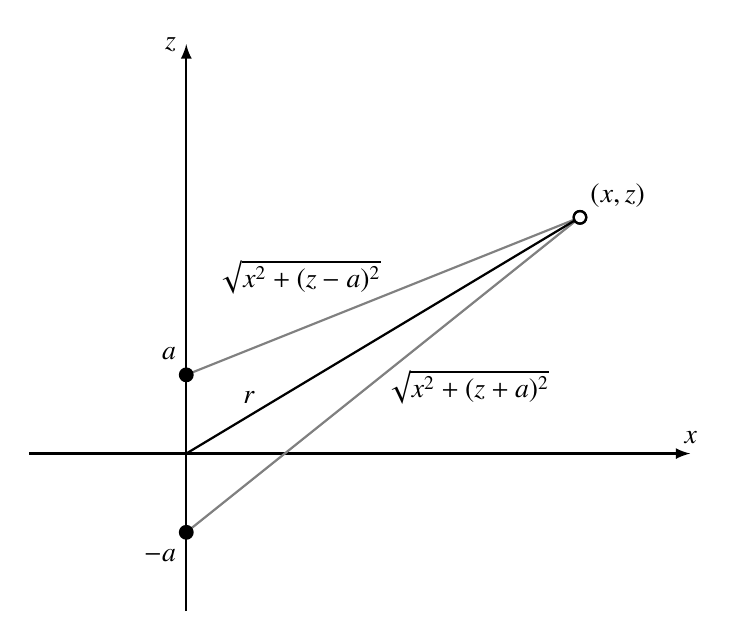
\begin{tikzpicture}[>=latex, thick, scale=2]

\draw[->] (-1,0)--(3.2,0) coordinate[label={above:$x$}];
\draw[->] (0,-1)--(0,2.6) coordinate[label={left:$z$}];

\node at (0,-0.5) [below left] {$-a\mathstrut$};
\node at (0, 0.5) [above left] {$\mathstrut a$};

\node at (0.5,0.25) [above left] {$r$};

\draw[gray] (0,0.5)--(2.5,1.5);
\draw[gray] (0,-0.5)--(2.5,1.5);

\draw (0,0)--(2.5,1.5);

\draw[fill=black] (0,-0.5) circle[radius=0.4mm,fill]{};
\draw[fill=black] (0,+0.5) circle[radius=0.4mm,fill]{};

\node at (1.3,0.95) [above left] {$\sqrt{x^2+(z-a)^2}$};
\node at (1.2,0.6) [below right] {$\sqrt{x^2+(z+a)^2}$};

\node at (2.5,1.5) [above right] {$(x,z)$};

\draw[fill=white] (2.5,1.5) circle[fill=white,radius=0.4mm]{};
\draw (2.5,1.5) circle[fill=white,radius=0.4mm]{};

\end{tikzpicture}
\end{document}
